
\chapter{MPMICE} \label{Sec:MPMICE}

\section{Introduction}

MPMICE is a marriage of the multi-material ICE method, described in
Section~\ref{Sec:ICE} and MPM, described in Section~\ref{Sec:MPM}.
The equations of motion solved for both fluid and solid are essentially
the same, although the physical behavior of these two states of matter
differ, largely due to their constitutive relationships.  MPM is used
to track the evolution of solid materials in a Lagrangian frame of
reference, while fluids are evolved in the Eulerian frame.

\section{Theory - Algorithm Description}

At this time, the reader is directed to the manuscript by Guilkey,
Harman and Banerjee~\cite{fourthmit} for the theoretical and algorithmic
description of the method.

%\subsection{Uintah Specification}

%\subsubsection{ICE}

%\subsubsection{Basic Inputs}
%\subsubsection{Physical Constants}
%\subsubsection{Material Properties}
%\subsubsection{Equation of State}
%\subsubsection{Exchange Properties}
%\subsubsection{BoundaryConditions}
%\subsubsection{Solvers}


%\subsection{MPM}

%\subsubsection{Basic Inputs}
%\subsubsection{Physical Constants}
%\subsubsection{Material Properties}
%\subsubsection{Constitutive Models}
%\subsubsection{Contact}
%\subsubsection{BoundaryConditions}
%\subsubsection{Physical Boundary Conditions}

\section{Examples}

\subsection*{\center Mach 2 Wedge}
\addcontentsline{toc}{subsection}{Mach 2 Wedge}
\subsubsection*{\underline{Problem Description}}
This is a simulation of a symmetric $20^o$ wedge traveling through initially
quiescent air at Mach 2.0.  A shock forms at the leading edge of the
wedge and an expansion fan over its top.  Consultation of oblique shock
tables, e.g.~\cite{ref:Saad} (pp.308-309) reveals that the angle of the leading
shock compares quite well with the expected value.  In addition, this
simulation demonstrates a few other useful features of the fluid-structure
interaction capability.  In this case, the structure is rigid, and as
such, essentially provides a boundary condition to the compressible flow
calculation.  Furthermore, the geometry of the wedge is described via a
triangulated surface, rather than the geometric primitives usually used.
This allows the user to study flow around arbitrarily complex objects,
without the difficulty of generating a body fitted mesh around that object.

\subsubsection*{\underline{Simulation Specifics}}
\begin{description}
\item [Component used:] \hfill rmpmice (Rigid MPM-ICE)
\item [Input file name:] \hfill Mach2Wedge.ups
\item [Command used to run input file:]\hfill sus Mach2Wedge.ups
(Note: The files wedge40.pts and wedge40.tri must also be copied to
the same directory as sus.)

\item [Simulation Domain:]\hfill    0.25 x 0.0375 x 0.001 m

\item [Cell Spacing:]\hfill \\
.0005 x .0005 x .001 m (Level 0)

\item [Example Runtimes:] \hfill \\
 20 minutes   (1 processor, 3.16 GHz Xeon)\\

\item [Physical time simulated:] \hfill 0.3 milliseconds

\item [Associated visit session:] \hfill M2wedge.session

\end{description}

\newpage

\subsubsection*{\underline{Results}}

Figure~\ref{figwedge} shows a snapshot of the simulation.  Contour
plot depicts pressure and reflects the presence of a leading shock
and an expansion fan.
\begin{figure}
  \center
  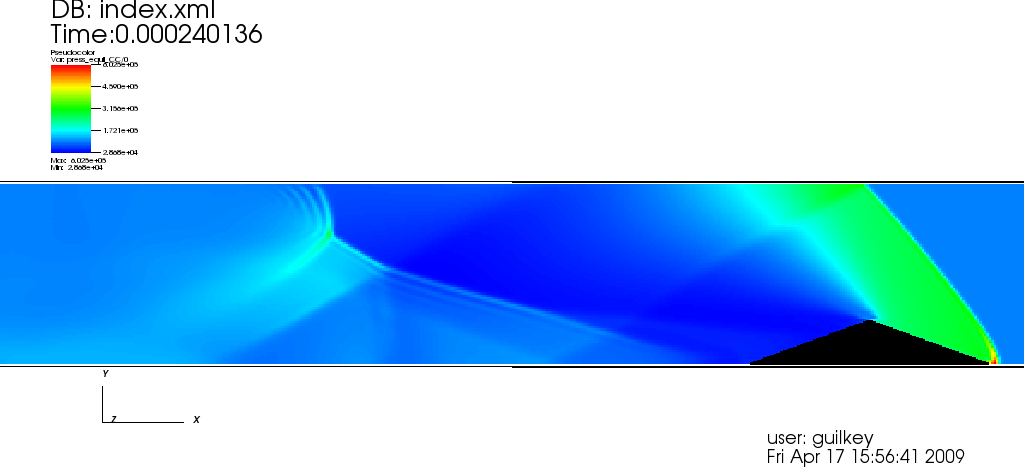
\includegraphics[scale=.4]{M2wedge.png}

  \caption{$20^o$ wedge moving at Mach 2.0 through initially stationary
air.  Contour plot depicts pressure.}
  \label{figwedge}
\end{figure}
\newpage
%
%__________________________________
\subsection*{\center Cylinder in a Crossflow}
\addcontentsline{toc}{subsection}{Cylinder in a Crossflow}
\subsubsection*{\underline{Problem Description}}
In this example the domain is initially filled with air moving at a uniform velocity of $0.03m/s$  A ridgid cylinder $O.D. = 0.02m$ is placed $0.1m$ from the inlet and a passive scalar is injected into the domain through a $0.002m$ hole on in the inlet boundary of the domain.  A velocity perturbation is placed upstream of the cylinder to produce an instablity that will help trigger the onset of the K\'arm\'an vortex street.
%
\subsection*{\underline{Simulation Specifics}}
\begin{description}
\item [Component used:] \hfill rmpmice (Rigid MPM-ICE)
\item [Input file name:] \hfill \TT{cylinderCrossFlow.ups}
\item [Command used to run input file:]\hfill \\
\TT{mpirun -np 6  sus inputs/UintahRelease/MPMICE/cylinderCrossFlow.ups}

\item [Simulation Domain:]\hfill    0.3 x 0.15 x 0.001 m

\item [Cell Spacing:]\hfill \\
.00015 x .001 x .001 m (Level 0)

\item [Example Runtimes:] \hfill \\
 7ish hrs   (6 processor, 3.16 GHz Xeon)\\

\item [Physical time simulated:] \hfill 60 seconds

\item [Associated visit session:] \hfill cyl\_crossFlow.session

\end{description}

\section*{\underline{Results}}

Figure~\ref{fig:cylCrossFlow} shows a snapshot of the simulation at time $t=60sec$.  The contour
plot of the passive scalar shows the K\'arm\'an vortex street behind the cylinder at $Re=700$.
\begin{figure}
  \center
  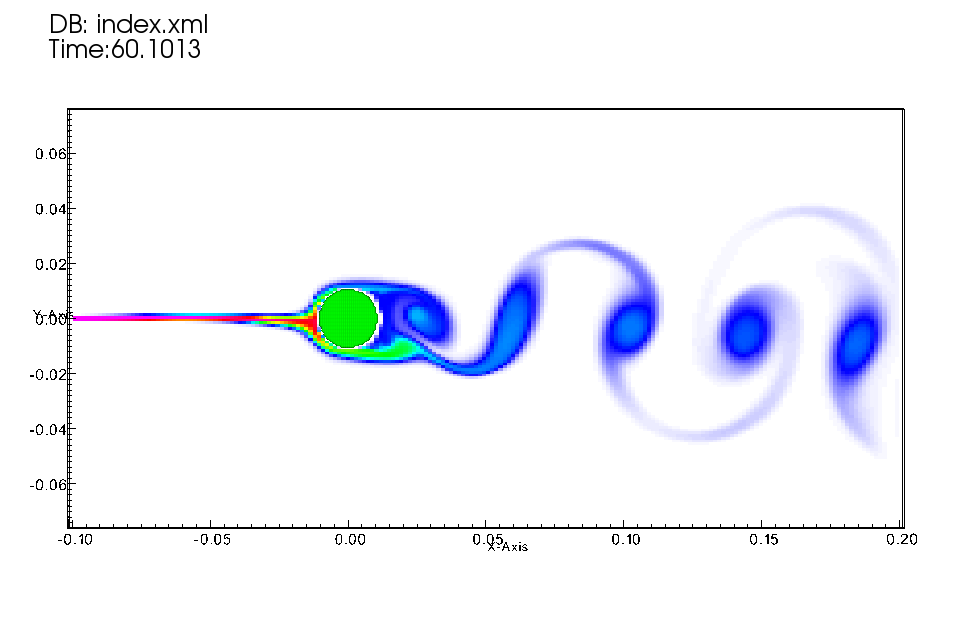
\includegraphics[scale=.5]{cylCrossFlow.png}
  \caption{Flow over a stationary cylinder, $Re=700$, a passive scalar is used as a flow marker}
  \label{fig:cylCrossFlow}
\end{figure}
%
A movie of the results is located at
\begin{Verbatim}[fontsize=\footnotesize]
  movies/cyl_crossFlow.mpg
\end{Verbatim}
\newpage

%__________________________________
\subsection*{\center Copper Clad Rate Stick (aka ``Cylinder Test")}
\addcontentsline{toc}{subsection}{"Cylinder Test"}
\subsubsection*{\underline{Problem Description}}

This is a two-dimensional version of the ``cylinder test" which is used to
characterize equations of state for explosive products.  In those tests, a
copper tube is filled with a high explosive and a detonation is initiated
at one end.  Various means are used to measure the velocity of the tube as
the high pressure product gases expand inside of it.

Here, a cylinder ($r=2.54 cm$) of QM100 is jacketed with a copper cylinder
that has a wall thickness of $0.52 cm.$   Detonation is initiated by giving
a thin layer of the explosive a high initial velocity in the axial direction
which generates a pressure that is sufficiently high to reach trigger the
detonation model.  As the detonation proceeds, the copper is pushed out of
the domain by the expanding product gases.

Note that in this example, to make run times brief, the domain is very short
in the axial direction, and is probably not sufficient for the detonation to
reach steady state.  Additionally, the domain has been reduced to two
dimensions, as symmetry is assumed in the Z-plane.  Finally, the spatial
resolution of $1.0 mm$ is a bit coarse to achieve 
convergent results.  The full three dimensional result can quickly be
obtained by commenting out the symmetry condition on the z+ plane and
uncommenting the Neumann conditions, as well as changing the spatial extents
and resolution in the Z direction to match those in the Y direction.

%
\subsubsection*{\underline{Simulation Specifics}}
\begin{description}
\item [Component used:] \hfill mpmice (MPM-ICE)
\item [Input file name:] \hfill \TT{QM100CuRS.ups}
\item [Command used to run input file:]\hfill \\
\TT{sus inputs/UintahRelease/MPMICE/QM100CuRS.ups}

\item [Simulation Domain:]\hfill    0.055 x 0.032 x 0.0005 m

\item [Cell Spacing:]\hfill \\
1.0 mm x 1.0 mm x 1.0 mm (Level 0)

\item [Example Runtimes:] \hfill \\
 20 minutes   (1 processor, 3.16 GHz Xeon)\\

\item [Physical time simulated:] \hfill 30 $\mu$seconds

\item [Associated visit session:] \hfill QM100.session

\end{description}

\subsubsection*{\underline{Results}}

Figure~\ref{fig:QM100} shows a snapshot of the simulation at time $t=60sec$.
Particles are colored by velocity magnitude, contours reflect the density of
explosive, note the highly compressed region near the shock front.
\begin{figure}
  \center
  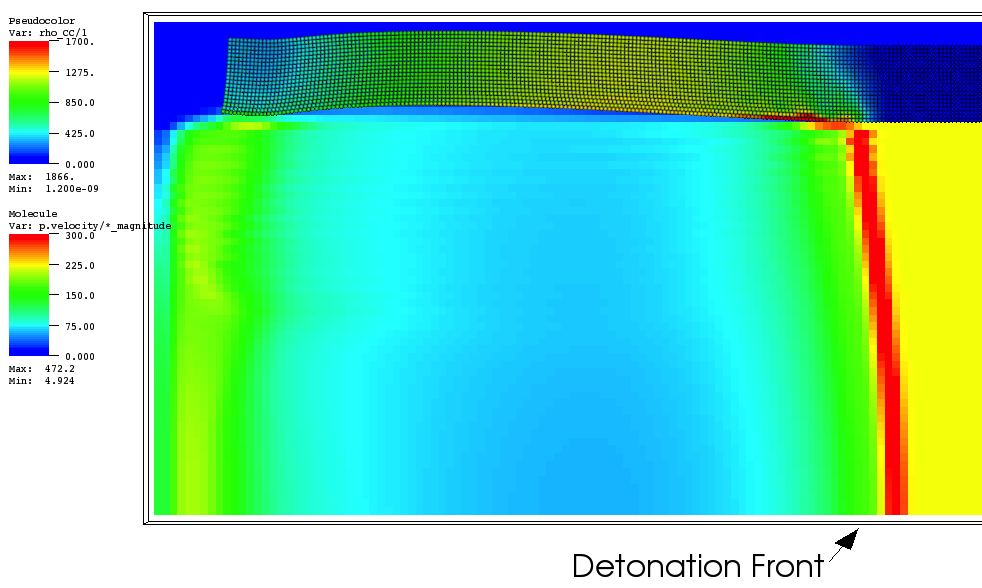
\includegraphics[scale=.5]{QM100.png}
  \caption{Detonation in a copper cylinder (2-D).  Particles are colored by
           velocity magnitude, contours indicate density of unreacted
           explosive.}
  \label{fig:QM100}
\end{figure}
%
\newpage

%
%__________________________________
\subsection{References}
\bibliographystyle{plain}
\bibliography{ice}
